\chapter{Kube Platform}
In this chapter, we commence on an in-depth exploration of the Kube platform, an implementation of
innovative ERP platform prototype. We start by outlining the fundamental requirements that have
shaped the development of the Kube platform, highlighting the strategic objectives, technical needs,
and business logic that inform its design. This leads us into a detailed examination of the
platform’s final architecture, which showcases a Microservices framework implemented through a
Function as a Service (FaaS) model, using AWS services. We then transition to practical
applications, where specific use cases demonstrate the platform's operational flow and its
real-world applicability. The chapter ends with a focus on the client application, delving into the
design and development of a user interface using Flutter, which not only complements the platform's
robust backend but also enhances the overall user experience. Throughout this chapter, we aim to
unravel the complexities of the Kube platform, illustrating its role as a transformative force in
the field of enterprise resource planning and highlighting its potential.

\section{Requirements}
Before starting development, requirements are established to define the properties of the product.
It's important that these requirements are thorough and coherent, covering all necessary features
without conflicts or inconsistencies. However, creating these documents can be challenging and
errors may occur, such as incomplete or ambiguous feature descriptions, redundancy, or important
details being omitted. To address these challenges, software engineering techniques have been
developed to formalize the requirements and minimize the occurrence of errors.
\newline\newline
ISO/IEC 25010\textsuperscript{\cite{ch5_1}}, an international standard, serves as a comprehensive
framework for assessing software product quality. This standard enumerates several key quality
characteristics, including functionality, reliability, usability, efficiency, maintainability,
security, compatibility, and portability. Its widespread application in software engineering and
quality assurance offers a standardized approach to evaluating and articulating software quality.
This facilitates more informed decisions in software acquisition, development, and maintenance.
ISO/IEC 25010 aids in identifying the actors involved and delineating both functional and
non-functional requirements.

\subsection{Stakeholders}
A stakeholder refers to any role, person, group, or organization that has an interest in a software
project or system being developed. This could include end-users, customers, investors, project
managers, developers and other individuals or groups involved in the development, deployment, and
maintenance of the software. Identifying all relevant stakeholders is important for considering
diverse perspectives and generating relevant requirements for the system. As shown in Table
\ref{tab:5_stakeholders}, numerous stakeholders play a role in the process.

\begin{table}[h]
    \centering
    \begin{tabular}{|l|p{10cm}|}
        \hline
        \textbf{Stakeholder} & \textbf{Description}                                                                                                                                                 \\ \hline
        End-users            & These are the people who will use the ERP system in their day-to-day work. They may include employees from various departments within the organization.              \\ \hline
        Developers           & These are the individuals responsible for creating the software code that makes up the ERP system.                                                                   \\ \hline
        Admin/IT staff       & These are the individuals responsible for installing, configuring, and maintaining the ERP system.                                                                   \\ \hline
        Customers            & These are the organizations or businesses that are purchasing the ERP system. They have a vested interest in ensuring the system meets their needs and requirements. \\ \hline
        Vendors              & These are the organizations that provide the ERP software and related services, such as installation, configuration, and support.                                    \\ \hline
        Cloud Vendors        & These hosts the system and provide the necessary infrastructure for its operation. They are responsible for system availability, scalability, and security.          \\ \hline
    \end{tabular}
    \caption{Stakeholders of a Cloud ERP System.}
    \label{tab:5_stakeholders}
\end{table}

\subsection{Functional and Non-functional}
Functional requirements and non-functional requirements are two types of requirements that are used
to specify what a system or software application should do and how it should perform. They are
important for the successful development and implementation of a system or software application. The
functional requirements ensure that the software application meets the needs of its users, while the
non-functional requirements ensure that the system is reliable, efficient, and secure.

\subsubsection{Functional requirements}
Functional requirements describe what the system should do in terms of its functionalities,
features, and capabilities. They define the specific tasks that the software application should be
able to perform to meet the needs of its users. For distinguish one requirement from another it is
important to assign for each functionality an ID, in order to easy identify it and trace throughout
the life cycle of the project (Table \ref{tab:functional_requirements}).

\begin{table}
    \centering
    \begin{tabular}{|l|p{10cm}|}
        \hline
        ID     & Description                                           \\ \hline
        FR1    & Sign-up users by email and password                   \\ \hline
        FR2    & Login users by email and password                     \\ \hline
        FR3    & Logout users                                          \\ \hline
        FR4    & Activate notifications                                \\ \hline
        FR5    & Deactivate notifications                              \\ \hline
        FR6    & View chart for andamento mensile degli ordini         \\ \hline
        FR7    & View chart for distribuzione degli ordini per cliente \\ \hline
        FR8    & Customize the menu bar                                \\ \hline
        FR9    & View the log of the platform events                   \\ \hline
        FR9.1  & View the detailed log of an event                     \\ \hline
        FR9.2  & Delete a log event                                    \\ \hline
        FR10   & View the customers list                               \\ \hline
        FR10.1 & View the detailed customer                            \\ \hline
        FR10.2 & Insert a customer                                     \\ \hline
        FR10.3 & Update a customer                                     \\ \hline
        FR10.4 & Delete a customer                                     \\ \hline
        FR11   & View the sales order list                             \\ \hline
        FR11.1 & View the detailed sales order with sales lines        \\ \hline
        FR11.2 & Insert a sales order                                  \\ \hline
        FR11.3 & Update a sales order                                  \\ \hline
        FR11.4 & Delete a sales order                                  \\ \hline
        FR11.5 & Insert a sales order line                             \\ \hline
        FR11.6 & Update a sales order line                             \\ \hline
        FR11.7 & Delete a sales order line                             \\ \hline
        FR12   & Launch the posting order event                        \\ \hline
        FR13   & show notifications of change status on order          \\ \hline
        FR14   & View the shipment list                                \\ \hline
        FR14.1 & View the detailed shipment with sales lines           \\ \hline
        FR14.2 & Delete a shipment                                     \\ \hline
        FR15   & View the invoice list                                 \\ \hline
        FR15.1 & View the detailed invoice with sales lines            \\ \hline
        FR15.2 & Delete an invoice                                     \\ \hline
    \end{tabular}
    \caption{Functional requirements for the platform.}
    \label{tab:functional_requirements}
\end{table}

\subsubsection{Non-functional requirements}
Non-functional requirements describe how the system should perform in terms of its functionality,
reliability, usability, efficiency, maintainability, security, compatibility, and portability, all
aspects that are not directly related to the specific functionalities to be implemented. They refer
to operating methods and constraints, such as response times, supported platforms, choice of
languages, required resources, tools and various implementation techniques. They must be measurable
and may be more critical than functional requirements. They are identified with a unique code and it
is also necessary to specify their type associated to the ISO properties and which functional
requirements they refer to (Table \ref{tab:non_functional_requirements}).

\begin{table}
    \centering
    \begin{tabular}{|l|c|p{9cm}|}
        \hline
        ID   & Type            & Description                                                        \\ \hline
        NFR1 & Usabilty        & Application should be used with no training by any user            \\ \hline
        NFR2 & Efficiency      & All functions should complete in < 0.5 sec                         \\ \hline
        NFR2 & Efficiency      & All functions must optimize the resource utilization               \\ \hline
        NFR3 & Portability     & System must work on Chrome, Firefox, Safari, Edge, Android and iOS \\ \hline
        NFR4 & Portability     & No installation is needed                                          \\ \hline
        NFR5 & Compatibility   & Platform must be compatible with Azure and AWS cloud               \\ \hline
        NFR6 & Security        & All data must be stored in a secure database                       \\ \hline
        NFR7 & Maintainability & All functionalities must be tested indipendently                   \\ \hline
        NFR8 & Reliabilty      & Downtime allowed is of one hour per year                           \\ \hline
    \end{tabular}
    \caption{Non-functional requirements for the platform.}
    \label{tab:non_functional_requirements}
\end{table}

\section{Server application}
In this section, we will discuss the final architecture designed for the Kube platform, encompassing
its data structures and services. We will explore the database setup, highlighting the tables
crafted for each microservice. Following this, we'll shed light on the REST APIs tailored for every
microservice, along with the integration of queues and events designed for asynchronous event
management. Concluding our discussion, we'll outline a SAGA implementation that has been
incorporated into the platform.
\newpage

\subsection{Final Architecture}
\begin{figure}
    \centering
    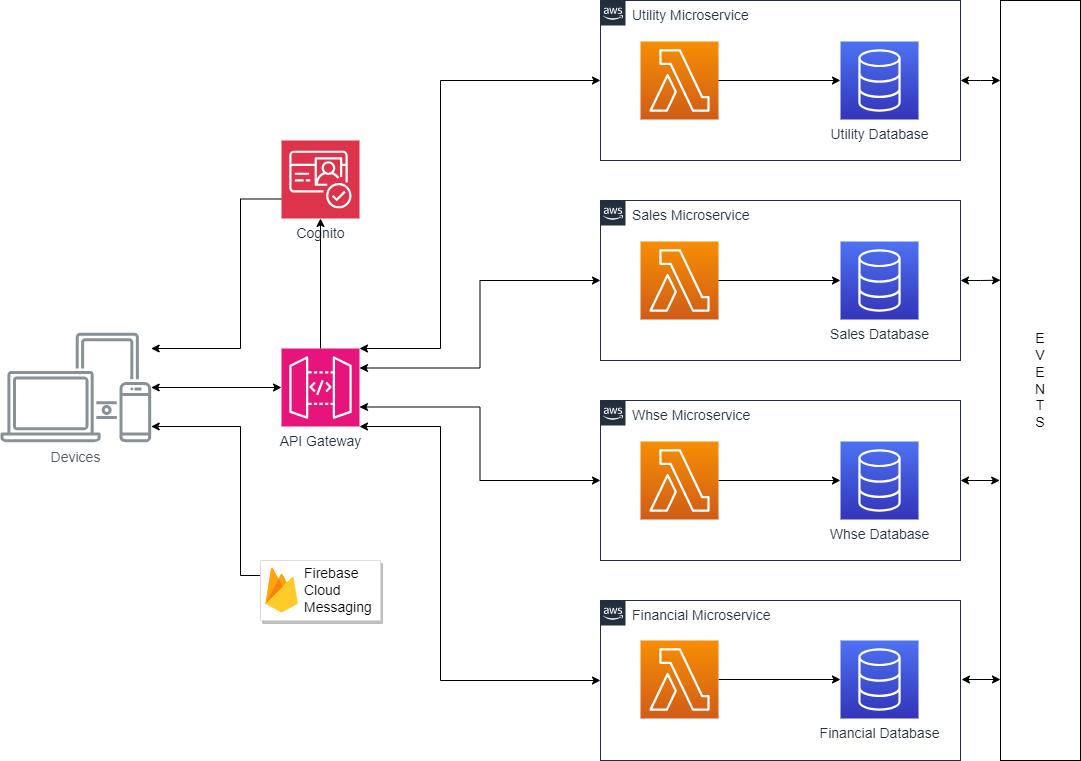
\includegraphics[scale=0.35]{Pictures/5_architecture2.png}
    \caption{Final architecture of the platform.}
    \label{fig:5_architecture}
\end{figure}
The architecture diagram in Figure \ref{fig:5_architecture} showcases a modern, serverless
microservices-based architecture for the Kube system. Here's a description based on the elements and
their interconnections:

\begin{itemize}
    \item \textbf{User Authentication}: the service which is responsible for user authentication is
          'Cognito'. It is the entry point for security, ensuring that only authenticated users can
          interact with the platform and with all the API.

    \item \textbf{Firebase Cloud Messaging}: At the bottom of the diagram, we can see 'Firebase Cloud Messaging',
          it is an integration with a cloud solution for sending notifications to devices, allowing for
          real-time user engagement.

    \item \textbf{API Gateway}: The 'API Gateway' is the central hub through which all client
          requests pass. It acts as a front door, directing incoming requests from various devices (such as
          computers and mobile phones) to the appropriate microservices.

    \item \textbf{Microservices Architecture}: Actually each microservice is deployed to AWS (Amazon
          Web Services), and utilize various AWS serverless features for optimizing performance.

          \begin{itemize}
              \item \textbf{Utility Microservice}: This service handles log functions and events,
                    and is backed by a 'Utility Database' for storing log records. It also manage
                    home page graph function and data and navigations/menu API and data.
              \item \textbf{Sales Microservice}: Dedicated to handling sales-related operations,
                    like handle customer and sales order, this service interacts with a 'Sales
                    Database'.
              \item \textbf{Whse Microservice}: this service manages shipment and warehouse-related
                    data, backed by its own 'Whse Database'.
              \item \textbf{Financial Microservice}: This handles financial transactions and invoice, with a
                    separate 'Financial Database' for storing related records.
          \end{itemize}

    \item \textbf{Database Pattern}: The architecture uses a database-per-microservice pattern with SQL
          databases, ensuring that each service has its own datastore, thus maintaining database isolation and
          decoupling services.

    \item \textbf{Event-Driven Architecture}: all microservices are connected through an
          event-driven architecture, which allows them to communicate asynchronously and facilitates
          loose coupling. This architecture is implemented using Amazon Simple Queue Service (SQS)
          and Amazon Simple Notification Service (SNS), which are managed message queues and
          notification services.
\end{itemize}

All services are managed and deployed using the serverless framework, which allows to easily
integrate a CI/CD pipeline manage the entire infrastructure as code. With this setup, the platform
can be easily deployed to other cloud providers and add other cloud services and features. How we
can see, the Kube platform's architecture is designed to be scalable, flexible, and maintainable,
with a focus on modern cloud-native principles and best practices for microservices development.

\subsubsection{Microservices components}
\begin{figure}
    \centering
    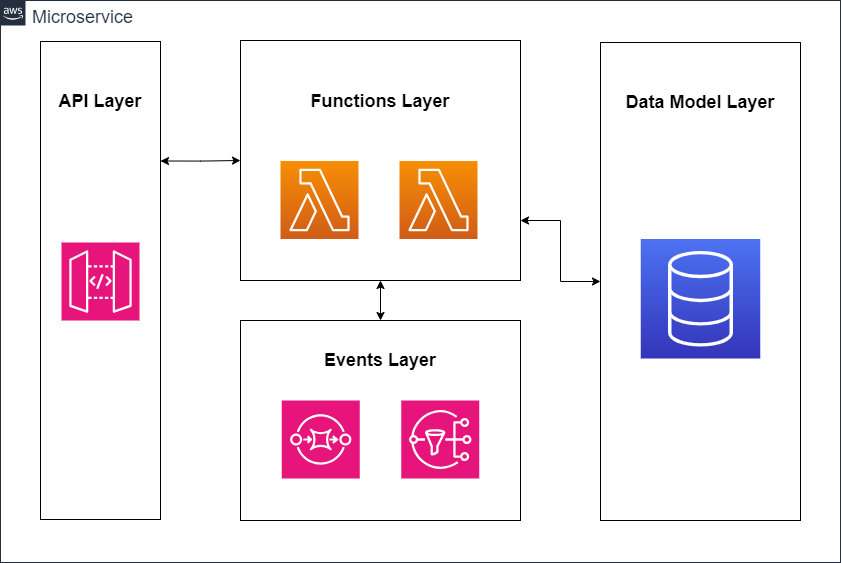
\includegraphics[scale=0.28]{Pictures/5_microservizio.png}
    \caption{Microservices components.}
    \label{fig:5_microservices}
\end{figure}

Each microservice in the Kube platform is a composite of four essential components that work in
concert to deliver its specific functionality:

\begin{table}
    \centering
    \begin{tabular}{|c|c|m{8.5cm}|}
        \hline
        \textbf{Component}   & \textbf{Service} & \textbf{Description}                                                                                                                                                                                                                                                                                                                                                                                                \\ \hline
        \textbf{Data Models} & RDS              & At the core of each microservice is a set of data models. These models define the structure of the data that the microservice handles, ensuring data integrity and consistency. By having its own models, each microservice encapsulates the necessary information to perform its tasks, leading to a clear delineation of responsibilities within the system.                                                      \\ \hline
        \textbf{REST APIs}   & API Gateway      & The REST APIs serve as the interfaces through which external services or client applications interact with the microservices. These APIs are carefully designed to provide a clear and consistent contract for accessing and manipulating data. They follow REST principles, allowing for stateless communication and enabling clients to perform standard HTTP operations such as GET, POST, PATCH, and DELETE.    \\ \hline
        \textbf{Functions}   & Lambda           & The functions are the operational units within each microservice, containing the business logic that processes requests, manipulates data models, and performs the necessary computations. These functions are likely implemented as serverless functions, which are executed in response to events, scaling automatically with the number of requests and reducing the need for managing server infrastructure.    \\ \hline
        \textbf{Events}      & SNS, SQS         & Each microservice also incorporates an event-driven mechanism, signaling and reacting to various conditions and triggers. These events facilitate asynchronous communication between microservices, thereby enhancing the platform's responsiveness and efficiency. By decoupling microservices through events, the system can better handle load variations and failure modes, contributing to overall resilience. \\ \hline
    \end{tabular}
    \caption{Microservices components.}
    \label{tab:microservices_components}
\end{table}

Together, these components create a modular and cohesive microservice that is self-contained,
scalable, and robust. The data models ensure that each service can independently manage its segment
of the data. The REST APIs provide the necessary endpoints for interaction, while the functions
encapsulate the business logic. Finally, the event system allows the services to react to and
communicate changes across the platform without direct coupling, promoting a reactive architecture
that can quickly adapt to changing conditions.
% eventually consistent is enough because not critical data and not all system is coupled

\subsection{Code Structure}
In our microservices architecture, all lambda functions are written in the Go language. This
decision was influenced by several key factors. Firstly, Go is a compiled language, which leads to
significantly faster execution times and results in smaller executable files. Another important
reason for choosing Go is the availability of the Go CDK library. This library is unique to Go and
aids in making functions as portable as possible across different cloud providers. While it's true
that shifting functions between providers requires some manual adjustments, the process could be
streamlined by developing CLI tools for automation.
\newline\newline
However, adopting Go was not without its challenges. Unlike object-oriented languages, Go doesn't
fully integrate all object-oriented principles. It has its own way of handling certain programming
concepts, which required a learning curve. Additionally, Go is not as versatile in some aspects; for
instance, the main function is bound to have a dedicated 'main' package. This can pose difficulties
in managing multiple functions, each with its own 'main,' making the overall management a complex
task.

\begin{figure}
    \centering
    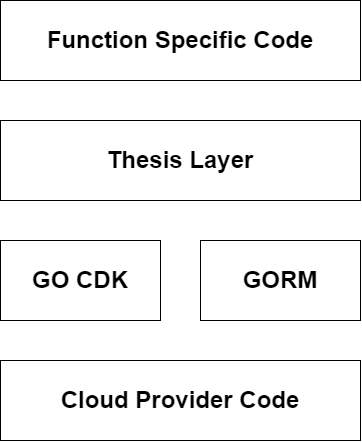
\includegraphics[scale=0.3]{Pictures/5_stack_framework.png}
    \caption{Stack abstractions layer.}
    \label{fig:5_stack_framework}
\end{figure}

In every function architecture, I've implemented an abstraction layer specifically designed for
managing REST APIs of various resources. This unified approach, applied across all microservices, is
facilitated by a layer we've named 'thesis.' Built on top of the GORM and Go CDK libraries, this
layer simplifies and accelerates API management. Connecting a GORM model to a 'thesis' layer
structure called 'page' requires minimal coding. The 'page' concept is central to our approach: it
automatically generates a suite of REST APIs for a resource, significantly reducing development time
and standardizing structures across resources. Moreover, these 'pages' can define a UI schema, which
clients can use to dynamically build pages for resources in their applications. The APIs that are
automatically constructed from a GORM model are structured as indicated inside the following tables.

\subsubsection{http://api.example.com/:pageid?field=value}
\begin{table}
    \centering
    \begin{tabular}{|m{2cm}|m{10cm}|}
        \hline
        \textbf{Method} & \textbf{Description}                                                                                                        \\ \hline
        \textbf{GET}    &
        Returns the list of records linked to the page. The records can be filtered by inserting the fields to be filtered in the URL's query string. \\ \hline
        \textbf{POST}   &
        Creates a new record in the table linked to the page.                                                                                         \\ \hline
        \textbf{PATCH}  &
        Edits the record in the table linked to the page.                                                                                             \\ \hline
        \textbf{DELETE} &
        Deletes records linked to the page. The records can be filtered by inserting the fields to be filtered in the URL's query string.             \\ \hline
    \end{tabular}
    \caption{REST API for page.}
    \label{tab:api_rest_1}
\end{table}

\subsubsection{http://api.example.com/:pageid/schema}
\begin{table}
    \centering
    \begin{tabular}{|m{2cm}|m{10cm}|}
        \hline
        \textbf{Method} & \textbf{Description}                     \\ \hline
        \textbf{GET}    &
        Returns the UI schema for building the page in the client. \\ \hline
        \textbf{POST}   &
        Not allowed.                                               \\ \hline
        \textbf{PATCH}  &
        Not allowed.                                               \\ \hline
        \textbf{DELETE} &
        Not allowed.                                               \\ \hline
    \end{tabular}
    \caption{Methods for page schema.}
    \label{tab:api_rest_2}
\end{table}

\subsubsection{http://api.example.com/:pageid/button?button\_id=value}
\begin{table}[!ht]
    \centering
    \begin{tabular}{|m{2cm}|m{10cm}|}
        \hline
        \textbf{Method} & \textbf{Description}                                   \\ \hline
        \textbf{GET}    &
        Initiates the functionality linked to the button and returns the result. \\ \hline
        \textbf{POST}   &
        Not allowed.                                                             \\ \hline
        \textbf{PATCH}  &
        Not allowed.                                                             \\ \hline
        \textbf{DELETE} &
        Not allowed.                                                             \\ \hline
    \end{tabular}
    \caption{Methods for page buttons.}
    \label{tab:api_rest_3}
\end{table}

\subsection{Utility Microservice}
This microservice is responsible for managing the home page graph data, the navigation menu, and the
logging system. It is the first microservice to be deployed, as it have the entry points of the
client application. In this microservice there are three crucial componentes of the platform: the
home page, the logging system and the navigation functionalities.

\subsubsection{Home Page}
The home page is the first page that the user see when he log in the client application. It is
composed by two graphs, one for the monthly trend of the orders and one for the distribution of the
orders by customer. The data of these graphs are stored in the database of the microservice and are
updated by the final event of the posting order chain, it call the graph update function. The home
page is implemented by a page model, so through a Lambda function, which is triggered by HTTP API by
the client. The Lambda function is responsible for updating the home page table.

\subsubsection{Logging System}
The logging component allows for monitoring and debugging the system. It is implemented through a
FIFO Queue, using Amazon SQS, and a Lambda function, which is triggered by the queue. The Lambda
function is responsible for writing the log to the database of the microservice, inside the Log
tabel. Thanks to the thesis layer in the framework stack, a message to the logging queue is
automatic sended when an error occurs in the platform (even in other microservices).

\subsubsection{Navigation}
The navigation component is responsible for managing the menu bar of the client application. It have
a list of all the page ids that most be present in the client menu bar. This list is stored in the
table navigation and is updated by the client application when the user customize the menu bar.
It not have only ids information but also the order of the pages in the menu bar, the icon to show,
the caption name to show and the entry point of the page. The entry point is the url of the page
that the client application must call when the user click on the page in the menu bar, and it depends
on the microservice that manage the page. The navigation component is implemented by a page model, so
through a Lambda function, which is triggered by an HTTP API by the client. The Lambda function is
responsible for updating the navigation table.

\subsubsection{Functions}
In the table \ref{tab:5_utility_functions} are summarized all the lambda functions of the utility
microservice, with the relative description and the trigger event (type and name).

\begin{table}
    \centering
    \begin{tabular}{|l|c|l|m{5.5cm}|}
        \hline
        \textbf{Name}  & \textbf{Type} & \textbf{Event Name} & \textbf{Description}                             \\ \hline
        Home           & API           & /home               & handle home page GET request                     \\ \hline
        GraphUpdate    & SNS           & OnFinishPostOrder   & Update graph data for home page                  \\ \hline
        NavigationList & API           & /navigationlist     & represents the list page of navigation model     \\ \hline
        NavigationCard & API           & /navigationcard     & represents the detailed page of navigation model \\ \hline
        LogList        & API           & /loglist            & represents the list page of log model            \\ \hline
        LogCard        & API           & /logcard            & represents the detailed page of log model        \\ \hline
        LogMessage     & SQS           & LogMessageQueue     & for logging the message in RDS database          \\ \hline
    \end{tabular}
    \caption{Functions of utility microservice.}
    \label{tab:5_utility_functions}
\end{table}

% TODO aggiungere le tabelle?

\subsection{Sales Microservice}
This microservice is specifically designed to handle and manage customer and sales order data. It
includes dedicated page functionalities that allow for efficient management and access to both
customer and sales order information. The data related to these entity are securely stored in a
specialized database, named 'sales', which is an integral part of this microservice. Additionally,
this service is equipped with a lambda function that plays a crucial role in orchestrating the saga
of posting orders. This function ensures that the process of managing and posting sales orders is
conducted smoothly and effectively.

\subsubsection{Functions}
In the table \ref{tab:5_sales_functions} are summarized all the lambda functions of the sales
microservice, with the relative description and the trigger event (type and name).

\begin{table}
    \centering
    \begin{tabular}{|l|c|l|m{4.3cm}|}
        \hline
        \textbf{Name}      & \textbf{Type} & \textbf{Event Name}    & \textbf{Description}                                                                               \\ \hline
        CustomerList       & API           & /customerlist          & represents the list page of customer model                                                         \\ \hline
        CustomerCard       & API           & /customercard          & represents the detailed page of customer model                                                     \\ \hline
        SalesOrderList     & API           & /salesorderlist        & represents the list page of sales order model                                                      \\ \hline
        SalesOrderCard     & API           & /salesordercard        & represents the detailed page of sales order model, it has the button for start the posting process \\ \hline
        SalesOrderLineList & API           & /salesorderlinelist    & represents the list page of sales order lines                                                      \\ \hline
        SalesOrderLineCard & API           & /salesorderlinecard    & represents the detailed page of sales order lines                                                  \\ \hline
        ChangeOrderStatus  & SQS           & ChangeOrderStatusQueue & the function that orchestrates the saga                                                            \\ \hline
    \end{tabular}
    \caption{Functions of sales microservice.}
    \label{tab:5_sales_functions}
\end{table}


\subsection{Whse and Financial Microservice}
These two microservices are tailor-made to manage shipments and invoices, each equipped with its
respective page model and database. They incorporate lambda functions integral to the posting order
saga. These functions are tasked with creating shipments and invoices, as well as updating the
status of sales orders.

\subsubsection{Functions}
In the table \ref{tab:5_whse_financial_functions} are summarized all the lambda functions of the Warehouse
and Financial microservice, with the relative description and the trigger event (type and name).

\begin{table}
    \centering
    \begin{tabular}{|l|c|l|m{6cm}|}
        \hline
        \textbf{Name} & \textbf{Type} & \textbf{Event Name} & \textbf{Description}                                                 \\ \hline
        ShipmentList  & API           & /shipmentlist       & represents the list page of shipment model                           \\ \hline
        ShipmentCard  & API           & /shipmentcard       & represents the detailed page of shipment model                       \\ \hline
        PostShipment  & SNS           & OnPostShipment      & the function that create shipment and recall the change order status \\ \hline
        InvoiceList   & API           & /invoicelist        & represents the list page of invoice model                            \\ \hline
        InvoiceCard   & API           & /invoicecard        & represents the detailed page of invoice model                        \\ \hline
        PostInvoice   & SNS           & OnPostInvoice       & the function that create invoice and recall the change order status  \\ \hline
    \end{tabular}
    \caption{Functions of Whse. and Financial microservices.}
    \label{tab:5_whse_financial_functions}
\end{table}

\subsection{Posting Order Saga}
The posting order saga, designed for users to post sales orders, operates through a series of
orchestrated lambda functions. At its core is the 'ChangeOrderStatus' function from the sales
microservice, which manages the sequence of steps in the saga. This function is triggered by an SQS
queue, which initially receives data when a user clicks the 'Post Order' button via the
'SalesOrderCard' function. Once activated, the 'ChangeOrderStatus' function begins the saga, leading
to a sequence of lambda functions, each set off by an SNS event. Key functions in this saga include
'CreateShipment' from the warehouse microservice and 'CreateInvoice' from the financial
microservice. This well-organized method ensures a seamless and efficient process for posting
orders.

\begin{figure}
    \centering
    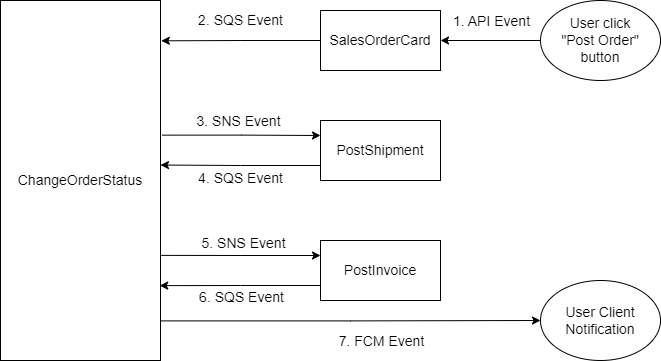
\includegraphics[scale=0.6]{Pictures/5_saga.png}
    \caption{Sequence diagram of the posting order saga.}
    \label{fig:5_posting_order_saga}
\end{figure}

The figure \ref{fig:5_posting_order_saga} shows the sequence diagram of the posting order saga.
Here's a detailed description of the steps involved:
\begin{enumerate}
    \item User initiates the process by clicking the "Post Order" button, which triggers an API
          event which is processed by the SalesOrderCard function.
    \item The SalesOrderCard places a message in an SQS queue, the ChangeOrderStatusQueue. It is a
          FIFO queue, ensuring that messages are delivered to the recipient in the same order they were
          received by the queue.
    \item ChangeOrderStatus make the check of posting order, change the status of order in "Pending
          Shipment" and triggers an SNS event on topic OnPostShipment.
    \item The SNS event invokes the PostShipment function. It create the shipment and send an SQS
          message on ChangeOrderStatusQueue.
    \item ChangeOrderStatus change the status of order in "Shipped" and triggers an SNS event on topic OnPostInvoice.
    \item The SNS event invokes the PostInvoice function. It create the Invoice and send an SQS
          message on ChangeOrderStatusQueue.
    \item Upon successful invoice creation, the status of order is changed in "Invoiced" and a final
          Firebase (FCM) event is triggered, sending a notification to the user client.
\end{enumerate}

\section{Client Application}
The Kube application client, a multifaceted and versatile platform, is constructed using Flutter, a
well-known cross-platform framework. This comprehensive solution seamlessly supplies a wide array of
platforms including Android, iOS, and Web, while also extending support to desktop environments like
Windows, MacOS, and Linux, albeit with a current limitation in notification capabilities. At its
core, the application smoothly integrates various robust systems and components, each playing a
pivotal role in its functionality and are described in the following sections. These integral
elements include a secure authentication system featuring a Cognito login page, an efficient state
management setup utilizing the Provider package, a dynamic routing mechanism powered by the GoRouter
package, a custom-made page builder tailored to specific needs, and a reliable notification system
implemented through Firebase Cloud Messaging, Figure \ref{fig:5_client_application}.

\begin{figure}
    \centering
    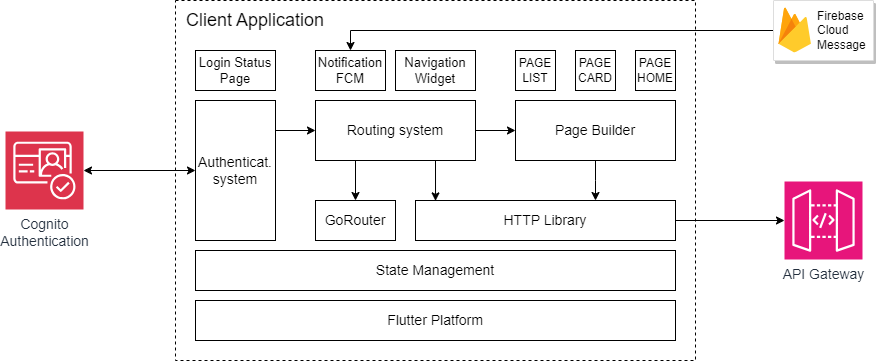
\includegraphics[scale=0.45]{Pictures/5_client.png}
    \caption{Client application architecture.}
    \label{fig:5_client_application}
\end{figure}

From an UI point of view, the application is designed to be simple and intuitive, with a clean and
modern look. Visually it is mainly composed of a menu bar and a page area, where the content of the
selected page is displayed. The Figure \ref{fig:5_client_UI} shows what the application
looks like.

\begin{figure}
    \centering
    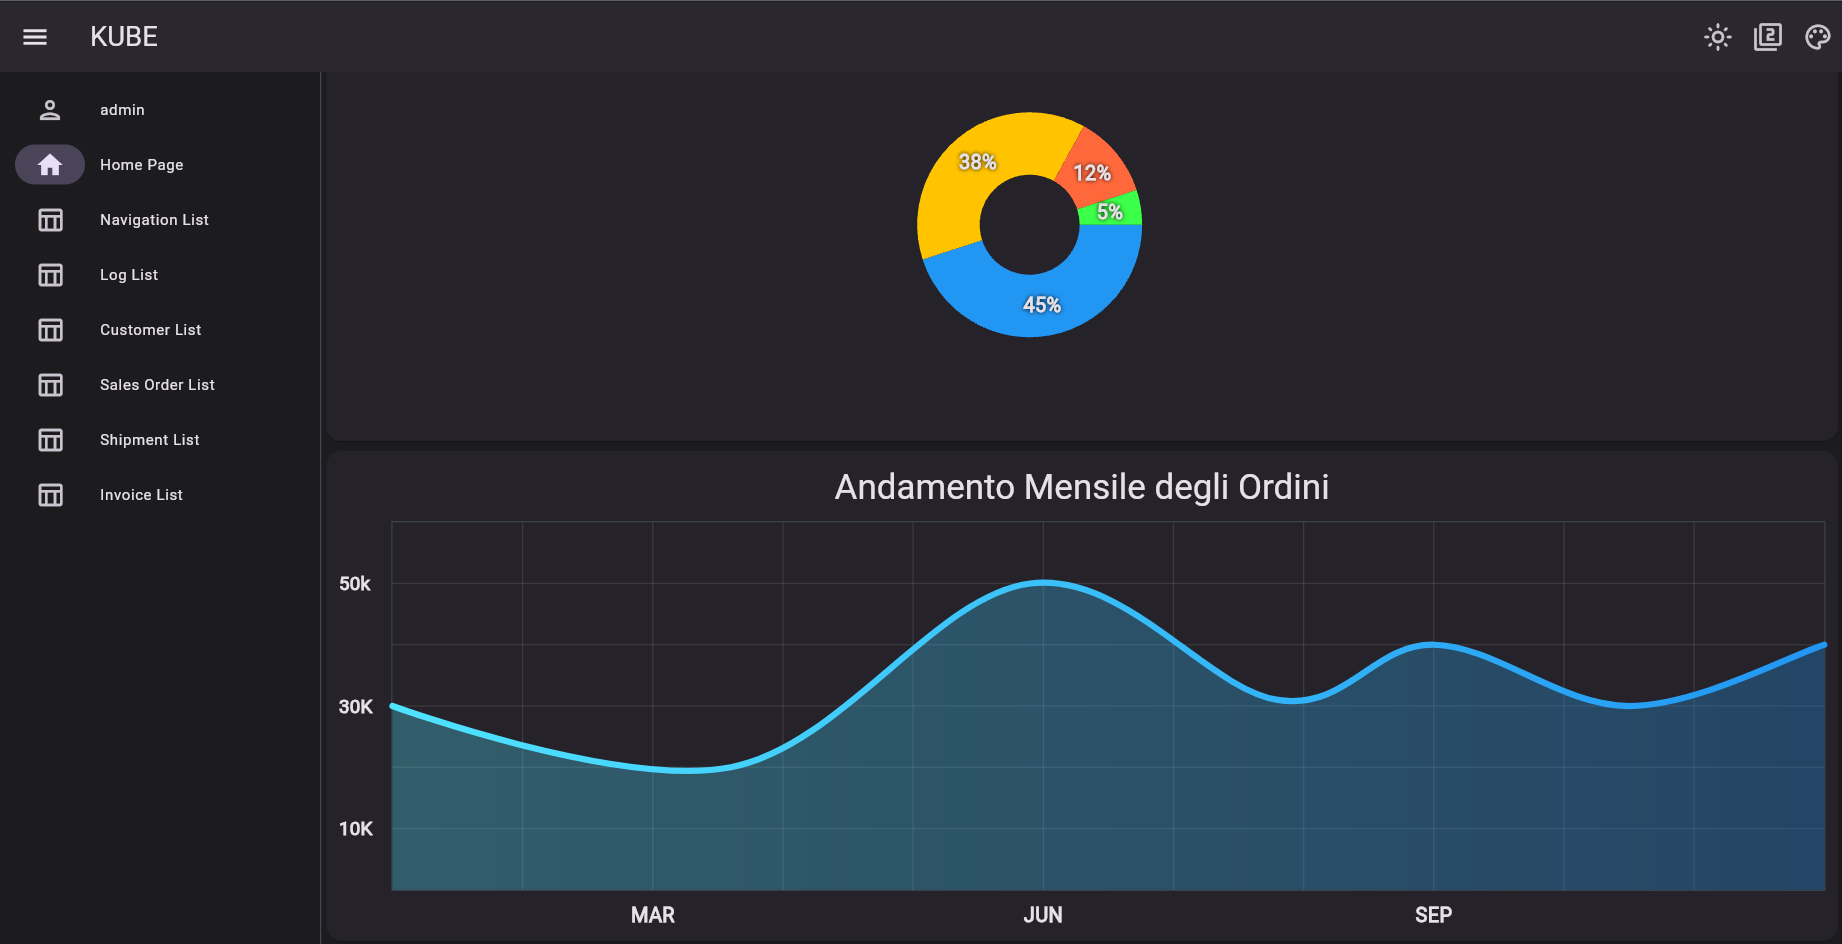
\includegraphics[scale=0.35]{Pictures/5_client_ui.png}
    \caption{Client UI.}
    \label{fig:5_client_UI}
\end{figure}

To enhance its effectiveness, the client application is hosted on GitHub Pages and is seamlessly
woven into a CI/CD pipeline orchestrated via GitHub Actions. This strategic implementation ensures a
streamlined deployment process: each commit to the repository triggers an automated build and
deployment sequence. This diligent approach guarantees that the latest iteration of the web
application is consistently accessible, embodying the epitome of efficiency and continuous
integration.

\subsection{State Management}
State management in the Flutter framework refers to the process of handling the data and UI states
of an app effectively. In Flutter, "state" can be anything that affects the UI and needs to be
tracked, such as user inputs, server responses, or even a timer's progress. Proper state management
ensures that the UI reflects the current state of the app accurately and efficiently, without
unnecessary rebuilds or updates. For the Kube application, the state is managed by the Provider
package. it is a popular library and it give an efficient way to manage state. It works by using a
mix of dependency injection and state management, allowing widgets to subscribe to changes in the
state of the app. Provider simplifies the process of passing data and events down the widget tree.
This approach not only makes the code more maintainable and scalable but also optimizes the app's
performance by rebuilding only those widgets that need to be updated. The figure
\ref{fig:5_provider} shows how the Provider package works.

\begin{figure}
    \centering
    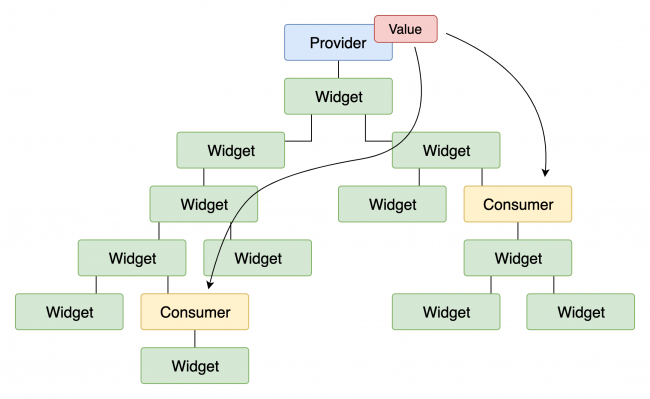
\includegraphics[scale=0.5]{Pictures/5_provider.png}
    \caption{Provider package.}
    \label{fig:5_provider}
\end{figure}

In this project, the Provider system is utilized for managing various states within the application.
It handles the user's authentication state, controls the navigation state of the menu bar, and
manages the notification state of the application, and finally it is used for handling the
controller page between several widgets on a single page.

\subsection{Authentication System}
The authentication system is a crucial component of the Kube application, ensuring that only
authenticated users can access the platform. This system is implemented using Amazon Cognito, a
comprehensive authentication service that provides secure user sign-up and sign-in functionality.
Cognito is a fully managed service, which means that it handles all the authentication processes,
including user registration, authentication, and account recovery.
\newline\newline
In this platform, the sign-up process is exclusively handled by the administrator, meaning that
users are unable to register themselves. Instead, users can only sign in using credentials provided
by the administrator. The authentication is facilitated through a Cognito login page, which is
accessible via the app's login page status - serving as the application's entry point. This process
is illustrated in Figure \ref{fig:5_auth}. Once authenticated, users gain access to the menu bar and
the various pages of the application, thereby unlocking the routing system which was previously
restricted.

% TODO fig:5_auth -> login state page -> cognito page -> menu bar unlocked -> interaction with page

\subsection{Routing System}
Kube application's routing system, an important aspect for page navigation, is powered by the
GoRouter package. This dynamic routing tool is both user-friendly and highly adaptable, supporting
custom routes and parameterized paths. Integrated state management ensures navigation state updates
in response to route changes, allowing the app to respond dynamically. The app features three
primary routes: login, home, and page, as shown in Table \ref{tab:5_routes}.

\begin{table}
    \centering
    \begin{tabular}{|l|l|m{7cm}|}
        \hline
        \textbf{Route} & \textbf{Page} & \textbf{Description}                                                                                      \\ \hline
        /login         & LoginStatus   & go to the page where are shown login information and login and logout buttons                             \\ \hline
        /home          & Home          & call the home API to retrieve page home information e show it                                             \\ \hline
        /page/:pageId  & Page Selected & open the page indicated in pageId parameter. Call the page API related and build the page based on schema \\ \hline
    \end{tabular}
    \caption{Routes and pages.}
    \label{tab:5_routes}
\end{table}

These routes are established in the main.dart file, the application's starting point. Positioned
under the navigation menu bar, which remains constantly visible, all routes are constructed
accordingly. Post-login, the first constructed widget is the menu bar, set up by querying the
navigation list API. This API, a GET request to the navigationlist function in the utility
microservice, retrieves a list of all pages to be displayed in the menu bar, with the relative icon,
caption and url. When a user interacts with the menu bar by clicking on its buttons, it initiates a
change in the application's navigation state. This action prompts the menu bar to be reconstructed.
In the menu, each button corresponds to a different page within the application. Therefore,
selecting a button results in a change to the respective page route, which in turn triggers the
refreshing of that page.

\subsection{Page Builder}
The Page Widget in our application is a custom-built, dynamic component that creates pages according
to a JSON schema fetched from the page API. Its design is intentionally flexible, allowing for the
construction of a variety of page types. The widget uses a switch statement to decide the type of
page to construct, based on the 'page type' defined in the schema. Currently, it supports three
types of pages: list, card, and home. The Figure \ref{fig:5_page_builder} is how the page builder
workflow operates:

\begin{figure}
    \centering
    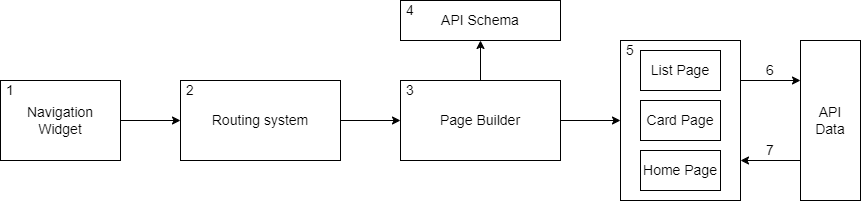
\includegraphics[scale=0.47]{Pictures/5_page_builder.png}
    \caption{Page builder workflow.}
    \label{fig:5_page_builder}
\end{figure}

\begin{enumerate}
    \item The User clicks on a menu bar button, triggering a change in the navigation state.
    \item The menu bar call the routing system to change the page with the pageId of the selected
          button.
    \item The Page Widget is initiated with a specific 'pageId' parameter.
    \item It then calls the page API to obtain layout information using the endpoint
          '/:pageId/schema'. This schema, a JSON format, outlines the structure of the page.
    \item Based on this layout information, the widget builds the page. There are three distinct
          page types it can construct: list, card, and home. For each page type, a specialized
          widget is employed to build the page: PageList for lists, PageCard for cards, and PageHome
          for the home page.
    \item These widgets then call their respective APIs, using '/:pageId' endpoint, to fetch the
          data needed for display. For the PageCard, a key filter is applied to retrieve specific records.
    \item After receiving the data from the API, each widget finish to constructs the page,
          populating it with the relevant data.
\end{enumerate}

% 3 esempi di pagine in json?

\subsection{Notification System}
In Kube platform, the notification system is implemented through Firebase Cloud Messaging (FCM), a
robust cross-platform messaging solution that ensures the reliable delivery of messages and
notifications to client applications. FCM, a free service, supports messaging to devices using iOS,
Android, and Web applications, although it does not extend to desktop applications. I have
seamlessly integrated FCM into the global state management system of our application. This
integration simplifies accessing and managing notification states, enabling the client application
to receive notifications effortlessly. Each notification is displayed as a snackbar at the bottom of
the screen, effectively informing users about important events on the platform, such as status
updates on orders or the creation of new shipments. This feature enhances user engagement by keeping
them promptly informed.

\section{Use Case}
A use case comprises various scenarios connected by a shared user objective, serving to illustrate
how a system behaves under different circumstances when processing a request. Each use case should
specify the system as an opaque entity, the user type (often referred to as the actor) interacting
with the system, and the actor's functional objective achieved through the system. A single scenario
represents a series of steps outlining the interaction between a user and the system. Additionally,
each scenario requires a pre-condition that must be met before initiation and a post-condition
fulfilled upon completion. This section will present several use cases, demonstrating the range of
operations a user can execute on the platform.

\subsection{User interaction}
This use case is applicable to all entities of the platform that have a page list, so it is a
generic use case. In this example we will see how the user can interact with the customer list page.
We use the insert example, but the same steps are valid for the update and delete operations. The
table \ref{tab:5_user_interaction} shows the steps of the scenario.

\begin{table}
    \centering
    \begin{tabular}{|l|p{10cm}|}
        \hline
        \textbf{Actors involved} & User                                                                              \\
        \hline
        \textbf{Precondition}    & The user U has already authenticated to the system and opened the customer list   \\
        \hline
        \textbf{Post-condition}  & The user U has created a new customer for the ERP system                          \\
        \hline
        \textbf{Normal scenario} &
        \begin{enumerate}
            \item The user U clicks on the add button
            \item Insert valid data in the opened detailed page
            \item Confirm the creation of the new customer
        \end{enumerate}                                                           \\
        \hline
        \textbf{Variant}         & The user inserts a non-valid data and the system inform him with an error message \\
        \hline
    \end{tabular}
    \caption{User interaction scenario}
    \label{tab:5_user_interaction}
\end{table}


\subsection{Posting order}
This use case show how the user can post an order. The table \ref{tab:5_posting_order} shows the
steps of the scenario.

\begin{table}
    \centering
    \begin{tabular}{|l|p{10cm}|}
        \hline
        \textbf{Actors involved} & User                                                                                   \\
        \hline
        \textbf{Precondition}    & The user U has already authenticated to the system and opened the sales order card     \\
        \hline
        \textbf{Post-condition}  & The user U has posted a sales order, and created a shipment and invoice document       \\
        \hline
        \textbf{Normal scenario} &
        \begin{enumerate}
            \item The user U clicks on the Posting button
            \item The system check if the order is valid
            \item The system create the shipment document
            \item The system create the invoice document
            \item The system change the status of the order in "INV"
            \item The system send a notification to the user U with the result of the posting order
        \end{enumerate}                            \\
        \hline
        \textbf{Variant}         & The user inserts a non-valid data and the system inform him with an error notification \\
        \hline
    \end{tabular}
    \caption{User interaction scenario}
    \label{tab:5_posting_order}
\end{table}
